\subsection{Cross Sections as a function of the proton transverse momentum}
%Results in P$_{p T}$ }

The differential cross section as a function of P$_{p T}$ for interactions on the CH, C, H$_{2}$O, Fe, and Pb targets, respectively, are shown in Fig.~\ref{figure:xsec_proton_pt}. P$_{p T}$ is the magnitude of the  momentum of the proton transverse to the beam direction. Nuclear effects might be expect to smear this quantity out.   The uncertainties broken down by source for both the absolute cross sections and the cross section ratios as a function of P$_{p T}$ can be found in Fig.~\ref{fig:xsec_err_proton_pt}.

% tki_proton_pt xsecs
\begin{figure}[h]  
	\centering
   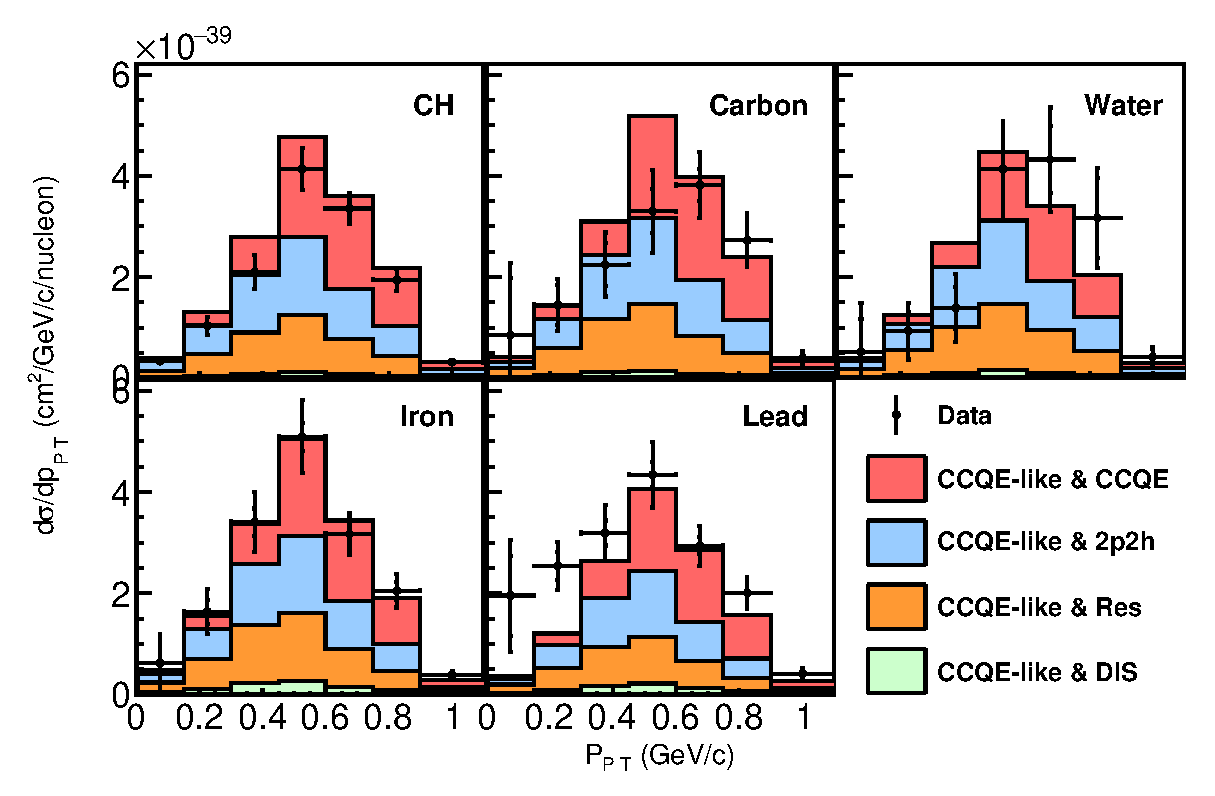
\includegraphics[width=\linewidth]{Figures/xsec_five_square/proton_pt.eps}
	\caption{The differential cross section as a function of P$_{p T}$ for CH, C, H$_{2}$O, Fe, and Pb targets, along with the predictions for the different quasielastic-like signal processes.}
	\label{figure:xsec_proton_pt}
\end{figure}

The data appear to be shifted to slightly higher P$_{p T}$ relative to the MINERvA tune simulation for the smaller nuclei. Fe is in good agreement.  For Pb, the distribution seems a little flatter than  the simulation, with more cross section at low P$_{p T}$ than expected.

The differential cross section as a function of P$_{p T}$ for the different targets as compared to a range of models is given in Fig.~\ref{fig:models_proton_pt}. The models all seem to peak at a slightly smaller P$_{p T}$ than is seen in the data for the smaller targets.  NEUT has a higher cross section than the data and this is particularly pronounced at low P$_{p T}$.  The hN versions of GENIE do this as well for the larger targets. Otherwise the models do a fairly good job describing the data.  The \chisq\ between the cross sections and the models can be found in Table~\ref{tab:protonpt}.

% comparisons to generators proton_pt
\begin{figure}
    \centering
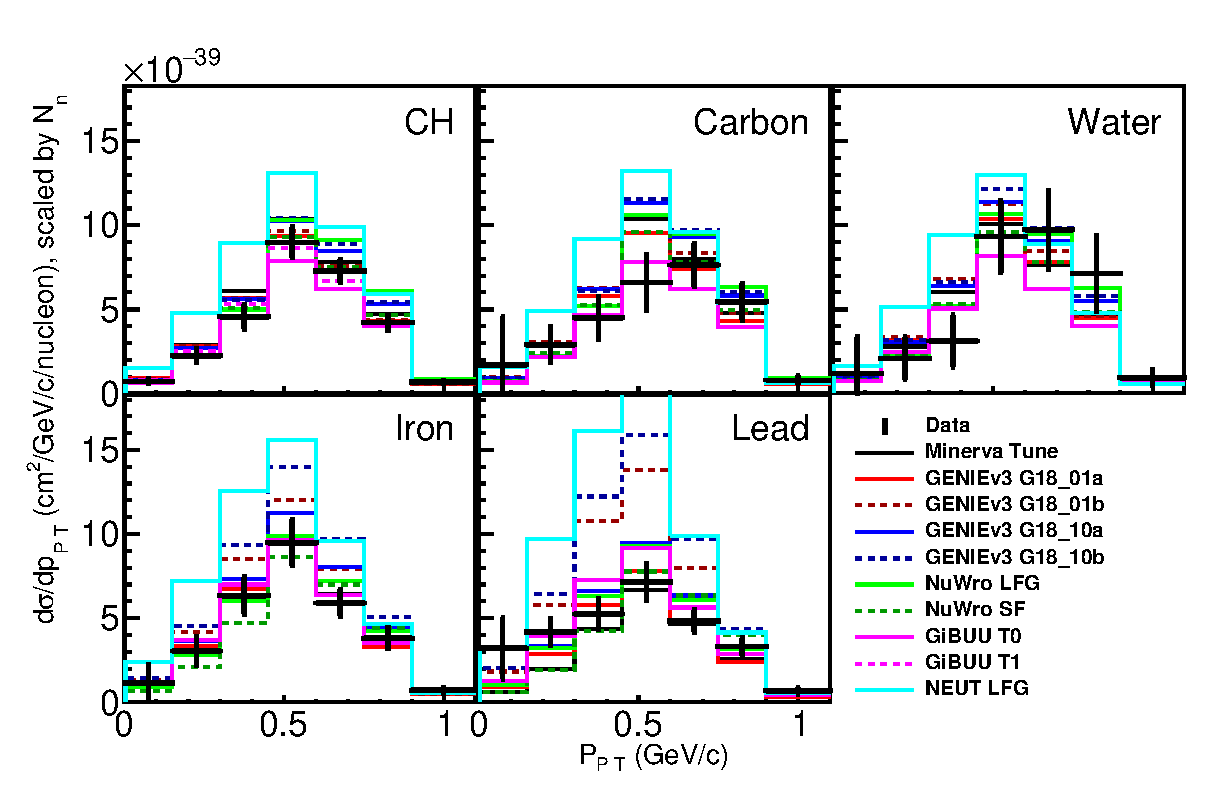
\includegraphics[width=\linewidth]{Figures/gencompare/proton_pt_5square.eps}
    \caption{Cross section measurements and predictions as a function of P$_{p T}$ for different targets and for a selection of different generator and model choices.}
    \label{fig:models_proton_pt}
\end{figure}

The ratio of the differential cross section as a function of  P$_{p T}$ for each nuclear target (C, H$_{2}$O, Fe, Pb) to that for scintillator is shown in 
Fig.~\ref{Figure:Gencompare_proton_pt_ratio}. The model spread becomes pronounced at low P$_{p T}$ for the Pb target.  At intermediate P$_{p T}$ in Pb, NEUT and the hN versions of GENIE have a higher ratio than the data. At lower P$_{p T}$ they agree with the data and most of the other models are lower, though the errors on the data are large.  GiBUU describes the data fairly well across targets and range in P$_{p T}$.  The \chisq\ between the cross section ratios and the models can be found in Table~\ref{tab:protonpt}.

\begin{figure}
    \centering
            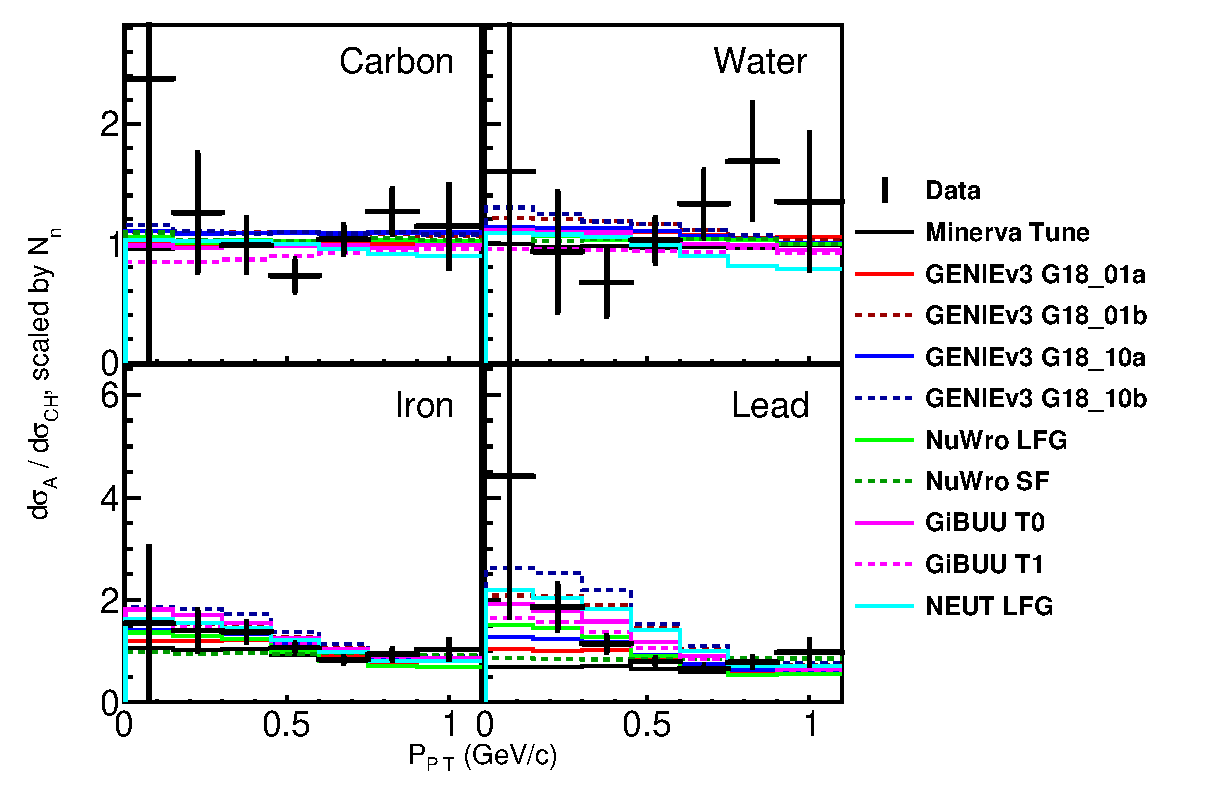
\includegraphics[width=\linewidth]{Figures/gencompare/proton_pt_4square.eps}
    \caption{Cross-section ratio as a function of proton transverse momentum, compared to several generators for multiple targets.  Changes to the FSI model (GENIE ``a'' to ``b'') in GENIE change the cross section ratio most at low proton angles, and those changes are larger than changes to the 2p2h model (GiBUU T0 to GiBUU T1) or changes to the initial state (GENIE 1 to GENIE 10) or (NuWro LFG to NuWro SF).}
        \label{Figure:Gencompare_proton_pt_ratio}
\end{figure}
